\documentclass{article}

\usepackage[english]{babel}
\usepackage{authblk}
\usepackage[a4paper,top=2cm,bottom=2cm,left=3cm,right=3cm,marginparwidth=1.75cm]{geometry}
\usepackage{amsmath}
\usepackage{graphicx}
\usepackage{gensymb}
\usepackage{textcomp}
\usepackage[backend=biber, style=apa, maxcitenames=1, uniquelist=false, url=false]{biblatex}
\usepackage{csquotes}
\usepackage[toc,page]{appendix}
\usepackage[colorlinks=true, allcolors=blue, breaklinks=true]{hyperref}
\usepackage{xurl}
\usepackage{multirow}
\usepackage{tabularx}
\usepackage{ltablex}
\usepackage{color}
\usepackage{tabularray}

\defbibenvironment{bibliography}
  {\begin{enumerate}}
  {\end{enumerate}}
  {\item}
\AtEveryBibitem{%
  \clearfield{note}%
}

% \AtEveryCitekey{\iffootnote{\csxdef{blx@footnotemark}{}\csxdef{blx@shortfootnotemark}{}}{}}

% \DeclareCiteCommand{\cite}
%   {\usebibmacro{prenote}}
%   {\usebibmacro{citeindex}%
%    \printtext[bibhyperref]{\usebibmacro{cite}}
%   }
%   {\multicitedelim}
%   {\usebibmacro{postnote}}

%   \DeclareCiteCommand{\parencite}
%   {\usebibmacro{prenote}}
%   {\usebibmacro{citeindex}%
%    \printtext[bibhyperref]{\bibopenparen\usebibmacro{cite}\bibcloseparen}
%   }
%   {\multicitedelim}
%   {\usebibmacro{postnote}}

% % Redefine \parencites to handle multiple citations in one set of parentheses
% \DeclareCiteCommand{\parencites}
%   {\usebibmacro{prenote}}
%   {\usebibmacro{citeindex}%
%    \printtext[bibhyperref]{\bibopenparen\usebibmacro{cite}\bibcloseparen}
%   }
%   {\multicitedelim}
%   {\usebibmacro{postnote}}

\addbibresource{references.bib}

\title{Predicting Ensemble Location and Width in Binaural Recordings of Music with Convolutional Neural Networks}
\author[1,*]{Paweł Antoniuk}
\author[1]{Sławomir Zieliński}
\affil[1]{Faculty of Computer Science, Białystok University of Technology}
\affil[*]{Corresponding author: pawel.antoniuk@sd.pb.edu.pl}
\date{}

\begin{document}
\maketitle


\begin{abstract}
  Binaural audio technology has been in existence for many years, but its popularity has significantly increased over the past decade as a consequence of advancements in virtual reality and streaming technologies. Along with its growing popularity, the quantity of publicly accessible binaural audio materials has also expanded. Consequently, there is now a need for automated and objective measurements of spatial content information, with ensemble location and width being the most prominent. This study presents a novel method for predicting ensemble location and width in binaural recordings of music. To this end, 30 head-related transfer functions and 192 binaural music recordings from publicly accessible multi-track recording repositories were used to synthesize 23,040 binaural recordings. The synthesized recordings were then used to train a multi-task convolutional neural network model, the aim of which was to predict the location and width of the ensemble for unseen recordings. The results indicate that models of ensemble location and width can be successfully constructed with low prediction errors --- $4.76\degree$ ($\pm0.10\degree$) for ensemble location and $8.57\degree$ ($\pm0.19\degree$) for ensemble width. The method developed in this study outperforms previous spatiogram-based methods recently published in the literature and holds promise for future development as a part of a novel tool for audio engineers to assess binaural audio.
\end{abstract}

\section{Introduction}

The human auditory system demonstrates exceptional proficiency in segregating, localizing, and interpreting diverse auditory signals, despite being limited to two ears. This is possible by internal examination of interaural differences in time, loudness, and frequency, known as binaural hearing \parencite{blauert_spatial_1996}, which enables precise localization of sound sources in complex auditory environments. A notable advantage of binaural hearing is exemplified by the `cocktail party effect', highlighting the system's capacity to concentrate on foreground sound sources while suppressing background noise \parencite{cherry_experiments_1953}. 

Understanding of the auditory system is essential for comprehending its limits and creating more immersive binaural experiences for entertainment purposes \parencite{zhang_surround_2017}. It is also important for enhancing auditory signal reception in hearing aid devices \parencite{hirsh_binaural_1950, thiemann_speech_2016}.

The advancement of sophisticated machine learning techniques, particularly deep learning networks, has prompted an intriguing exploration into the extent to which these tools can emulate the human auditory system. This exploration proceeds without reliance on the advanced spatial audio feature engineering traditionally used in audio source localization, as evidenced by some prominent recent examples \parencite{yang_deepear_2022, vera-diaz_towards_2018, pang_multitask_2019}. While the application of convolutional neural networks (CNNs) \parencite{lecun_handwritten_1989} --- traditionally employed in the visual domain --- to audio signals, particularly in conjunction with spectrograms \parencite{thomas_analyzing_2014, espi_exploiting_2015, han_convolutional_2017} or other feature engineering techniques \parencite{abdel-hamid_applying_2012, sainath_deep_2013}, is not novel. However, these approaches are continually being refined and adapted to the audio realm. Building on these foundations, this study developed an audio localization method by constructing a spectrogram-based multi-task CNN model.

Inspired by the fact, that humans tend to localize sound sources in groups rather than individually \parencite{bregman_auditory_1990, rumsey_spatial_2002}, the objective of the proposed model is to predict ensemble location and width instead of positions of individual sources. This study is unique as it not only conceptualized the method but also tested it on a vast, real-life music corpus of 23,040 binaural excerpts that were synthesized using 192 multi-track music recordings \parencite{senior_mixing_2023} and 30 publicly available head-related transfer functions (HRTFs) from various sources (see Table \ref{table:hrtfs} in \ref{appendix:a_hrtf}). The music recordings covered many different types of genres, including rock, jazz, pop, and classical music.

The findings demonstrate that this method is effective in accurately predicting the spatial characteristics of sound sources in near-real-world scenarios. Furthermore, this paper demonstrates an experimental framework that facilitates the objective measurement of a binaural localization technique, employing a large-scale dataset synthesized from real-world music signal (for applications of similar frameworks, see: \cite{antoniuk_blind_2023, zielinski_automatic_2022, zielinski_spatial_2022, zielinski_comparison_2020}). One of the key advantages of the proposed method is that it does not assume the number of audio sources. However, significant limitations of this study include the absence of reverberation in the synthesized recordings and the method's inapplicability to real-time scenarios --- both are critical areas for future research.

The developed method has the potential to be highly beneficial in automated assessment tasks, where a significant number of binaural recordings must be measured or labeled in terms of their spatial content information. This could be utilized in the development of a hypothetical autonomous web-crawler bot that will collect binaural recordings from publicly accessible repositories and label them according to the spatial properties of the sound sources, such as the location of the music ensemble or the sparsity of audio source positions. This method may also assist audio engineers in objectively assessing and segregating binaural audio recordings with regard to their spatial content.

The structure of this paper is organized as follows. Section \ref{sec:related-studies} presents related studies. The description of the method developed for this study is provided in Section \ref{sec:methodology}, which also includes detailed definitions of ensemble location and width, along with a description of the experiments used to evaluate this method. Section \ref{sec:results} presents and discusses the performance of the presented method and the results of the experiments conducted in this study. The paper concludes in Section \ref{sec:conclusions}.

\section{Related studies}
\label{sec:related-studies}

The majority of existing literature on the subject of sound source localization employs techniques that leverage the advantages of microphone arrays with more than two channels \parencite{kaveh_statistical_1986, pavlidi_real-time_2012, pan_multi-tone_2021, hahmann_sound_2022, chung_sound_2022, liu_sound_2022}. These method simplify the task and can improve the localization performance; however, they do not utilize binaural hearing, rendering them ineffective for binaural recordings.

In the context of sound source localization in binaural signals, the  focus of research is on the identification of individual sound sources, rather than groups of sounds \parencite{dietz_auditory_2011, may_probabilistic_2011, may_binaural_2012, woodruff_binaural_2012, may_robust_2015, ma16c_interspeech, ma_exploiting_2017, benaroya_binaural_2018}. In terms of source direction of arrival (DOA) methods, the majority of research assumes a fixed number of sound sources \parencite{pang_multitask_2019, vera-diaz_towards_2018, ma_exploiting_2017, woodruff_binaural_2012, arthi_spatiogram_2021}, which limits its practical applications as this information is rarely known in real-life binaural recordings. Moreover, the majority of studies have focused on relatively homogeneous signals, namely speech \parencite{dietz_auditory_2011, may_probabilistic_2011, may_binaural_2012, woodruff_binaural_2012, may_robust_2015, ma16c_interspeech, ma_exploiting_2017, benaroya_binaural_2018, wang_binaural_2020, liu_multiple_2018, yang_deepear_2022, ma_robust_2018}.

In contrast to the aforementioned studies, the proposed method is not constrained by the number of sources. Furthermore, the approach is not limited to speech and has been applied to a wide range of musical datasets, including instruments and vocals. In contrast to previous studies that primarily focused on individual sources, the proposed method does not aim to separate them, but rather considers them as a group, or in this case, a musical ensemble. This approach is similar to how the real musical ensembles are arranged on stage, thereby emphasizing practical applications in live settings. To the authors' knowledge, this is one of the first methods to localize ensemble width (see \cite{antoniuk_blind_2023} for the previous ensemble-width-related study), and the first to localize both ensemble position and width simultaneously using a multi-task model.


Sound localization methods can be classified into two categories based on the implementation of their underlying algorithms: glass-box (e.g., \parencite{dietz_auditory_2011, may_probabilistic_2011, may_binaural_2012, may_robust_2015, woodruff_binaural_2012, ma16c_interspeech, ma_exploiting_2017, ma_robust_2018}) and black-box (e.g., \parencite{vera-diaz_towards_2018, vera-diaz_towards_2018, yang_deepear_2022}). Glass-box methods, more traditional in the literature, rely on manually designed algorithms that mimic the auditory system to explicitly extract key features for location prediction, such as interaural level differences, interaural time differences, interaural coherence, or interaural phase differences (see \cite{blauert_spatial_1996} for feature descriptions). An example of one of the most advanced auditory models that is able to extract such features was developed by the Two!Ears project \parencite{raake_computational_nodate}.

In contrast, black-box methods generally employ minimal feature engineering, relying instead on advanced machine learning techniques to autonomously extract features and make predictions. These methods, while effective, do not explicitly reveal the features they extract nor necessarily mimic the human auditory system. This opacity and the unpredictable nature of the outcomes, coupled with their dependency on deep neural networks that have extensive learning parameters, require the use of very large datasets for development and evaluation. Such datasets often include thousands of examples, as seen in the TIMIT corpus with 6300 examples \parencite{garofolo_darpa_1993} used in multiple studies \parencite{yang_deepear_2022, benaroya_binaural_2018, wang_binaural_2020, vera-diaz_towards_2018, ma_exploiting_2017, pang_multitask_2019, ma_robust_2018, may_robust_2015}, or custom corpora comprising hundreds of thousands of recordings \parencite{antoniuk_blind_2023, zielinski_automatic_2022, zielinski_spatial_2022, zielinski_comparison_2020}. This poses a significant challenge in assembling a sufficiently large and diverse collection of labeled binaural recordings. However, this challenge can be addressed through the synthesis of binaural sounds, as demonstrated in various studies \parencite{antoniuk_blind_2023, zielinski_automatic_2022, zielinski_spatial_2022, zielinski_comparison_2020,yang_deepear_2022, ma_robust_2018} and further elaborated upon in Section \ref{subsec:synthesis} of this paper.

\section{Methodology}
\label{sec:methodology}

This section presents a detailed description of the main objective of the model developed as part of this study, as outlined in Section \ref{subsec:ensemble_definition}. It also describes the audio dataset used for training and evaluating the model, as detailed in Section \ref{subsec:synthesis}. In Section \ref{subsec:feature_extraction}, the feature extraction procedure is presented. Section \ref{subsec:topology} describes the model topology, whereas Section \ref{subsec:training_evaluation} address model training and evaluation.

\subsection{Ensemble location and width definition}
\label{subsec:ensemble_definition}

The objective of the model developed in this study is to predict the ensemble location ($\theta$) and width ($\omega$), as illustrated in Figure \ref{fig:scene}. An ensemble is defined as a group of audio point sources positioned on a circle around the listener on a virtual acoustic scene with equal distance to the listener. The location of source $i$ is denoted by $\theta_i$. The ensemble width ($\omega$) is defined as the angular width between two extreme point sources ($max_i(\theta_i)-min_i(\theta_i)$), while the ensemble location, designated by $\theta$, represents the middle angle between two extreme sound sources ($(max_i(\theta_i)+min_i(\theta_i))/2$). For the purposes of this study, the locations of the sources were limited to the frontal hemisphere only, i.e. $\theta\in[-45\degree, 45\degree]$, $\omega\in[0\degree, 90\degree]$, as this range encompasses the majority of real-world recording scenarios. It should be noted that although humans possess some limited abilities to localize sound sources in the vertical plane, in this study all sources are placed in the horizontal plane, at the height of the listener. This covers the majority of cases for real-world recordings (see \cite{ma_robust_2018, zielinski_spatial_2022} for related studies that cover top-down discrimination).

\begin{figure}[ht]
  \centering
  \includegraphics[width=\linewidth]{../pictures/scene.png}
  \caption{\label{fig:scene}Illustration of ensemble width ($\omega$) and ensemble location ($\theta$) that are relative to the direction of the head. Black dots represent the positions of audio sources $\theta_i$. The ensemble location ($\theta$) is defined as the angular position of the center of the ensemble relative to the direction the head is turned. The ensemble width ($\omega$) is defined as angular distance between two extreme audio sources. }
\end{figure}

\subsection{Synthesis of binaural music recordings}
\label{subsec:synthesis}

The experiments conducted in this study involved 23,040 binaural recordings of music. The binaural recordings were synthesized using 192 multi-track publicly-available music recordings \parencite{senior_mixing_2023} and 30 HRTF databases (see Table \ref{table:hrtfs} in \nameref{appendix:a_hrtf} for a detailed list of HRTF databases used in this study). The number of tracks in multi-track recording ranged from 5 to 62, with median of 9. For each pair of a multi-track recording and an HRTF database, four binaural recordings were synthesized with different random ensemble parameters, namely location $\theta$ and width $\omega$, as defined in Section \ref{subsec:ensemble_definition}. Both parameters were drawn from a uniform random distribution. Furthermore, the tracks of the input multi-track recordings were randomly assigned to sound source positions ($\theta_i$) to enhance the diversity of the final binaural corpora. Before the synthesis, the tracks were equalized to $-23$ LUFS, in accordance with the \parencite{noauthor_itu-r_2023} recommendation.

The binaural recordings were obtained in this study using the binaural synthesis procedure, known as binauralization, whose aim was to simulate the positions of sound sources within a virtual acoustic environment \parencite{blauert_spatial_1996}. This was achieved by convolving multi-track signals with head-related impulse responses from a specified head-related transfer function (HRTF) database. The resulting binaural output signal $y_c[n]$ for each stereo channel $c$ (left or right) at sample $n$ is given by the following equation:
\begin{equation}
  y_c[n] = \sum_{i=1}^{N} \sum_{k=0}^{K-1} x_i[k] \times h_{c,\theta_i}[n-k] ,
\end{equation}
where $x_i$ represents the signal of an individual sound source $i$ from the input music recording and $h_{c,\theta_i}$ denotes the head-related impulse response for channel $c$ at location $\theta_i$ of source track $i$.

Due to copyright restrictions, the music corpus utilized in this study was not published and can be provided upon request to the authors of this paper.

\subsection{Feature extraction}
\label{subsec:feature_extraction}

% The procedure proposed in this study did not 
% Zamiast tego dac obrazek z glowami i spektrogramami, lewy i prawi i roznica, sprawdzic czy to ma sens, potencjalnie usunac
% \begin{figure}[ht]
%   \centering
%   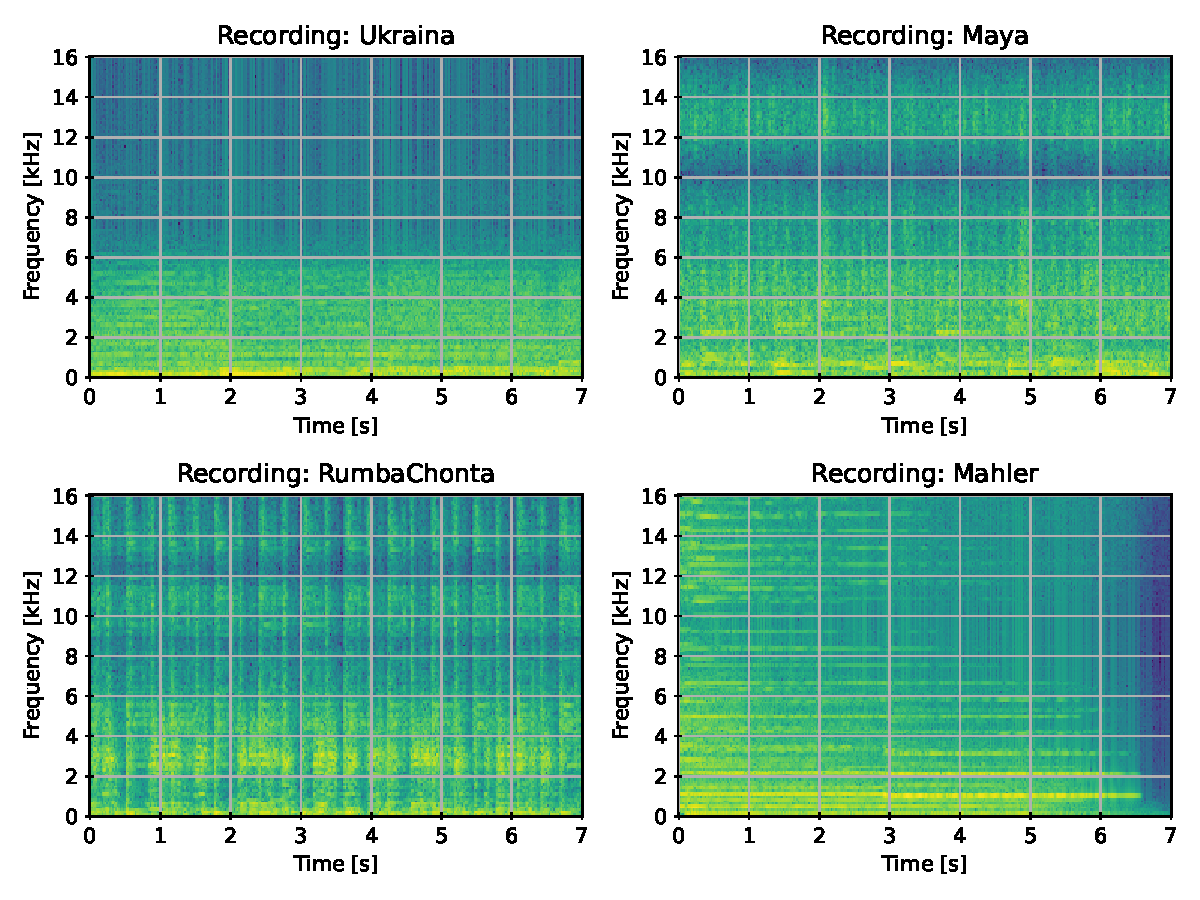
\includegraphics[width=\linewidth]{../figures/samples.pdf}
%   \caption{\label{fig:samples}Example magnitude spectrograms from randomly selected synthesized binaural music recordings, used as input data for training and evaluating the convolutional neural network (CNN) in this study. }
% \end{figure}
% Figure \ref{fig:samples} displays example spectrograms from four distinct binaural recordings, exhibiting a broad bandwidth and the diversity of the signals used in this study

Prior to input into the model, the binaural recordings of music were transformed into magnitude spectrograms. Although spectrograms do not directly provide information that can be translated into ensemble features, especially ensemble width, the goal of this task was to reduce the number of independent variables compared to the raw audio signal by extracting more compressed and informative data in the frequency domain. This step was necessary to decrease the likelihood of overfitting, reduce the number of examples needed to train the model, and thereby lower the overall computational power requirements. It is worth mentioning, however, that recent methods have shown that CNNs can be suitable for end-to-end audio localization without the spectrogram extraction step \parencite{vera-diaz_towards_2018, vecchiotti_end--end_2019}.

To prepare the input for the model, a Hamming window of 40 ms was applied to each frame of the signal, resulting in a total of 349 time frames. From each frame, spectrograms were extracted using the Fast Fourier Transform (FFT) algorithm, with 150 frequency bands spaced linearly from 100 Hz to 16 kHz. This procedure was conducted for both the left and right channels, yielding two spectrograms for each binaural sample. Consequently, each sample was represented by a floating-point precision matrix of dimensions $2 \times 349 \times 150$. This method parallels the procedure presented by \cite{zielinski_automatic_2022}.

\subsection{Network topology}
\label{subsec:topology}

\begin{figure}[ht]
  \centering
  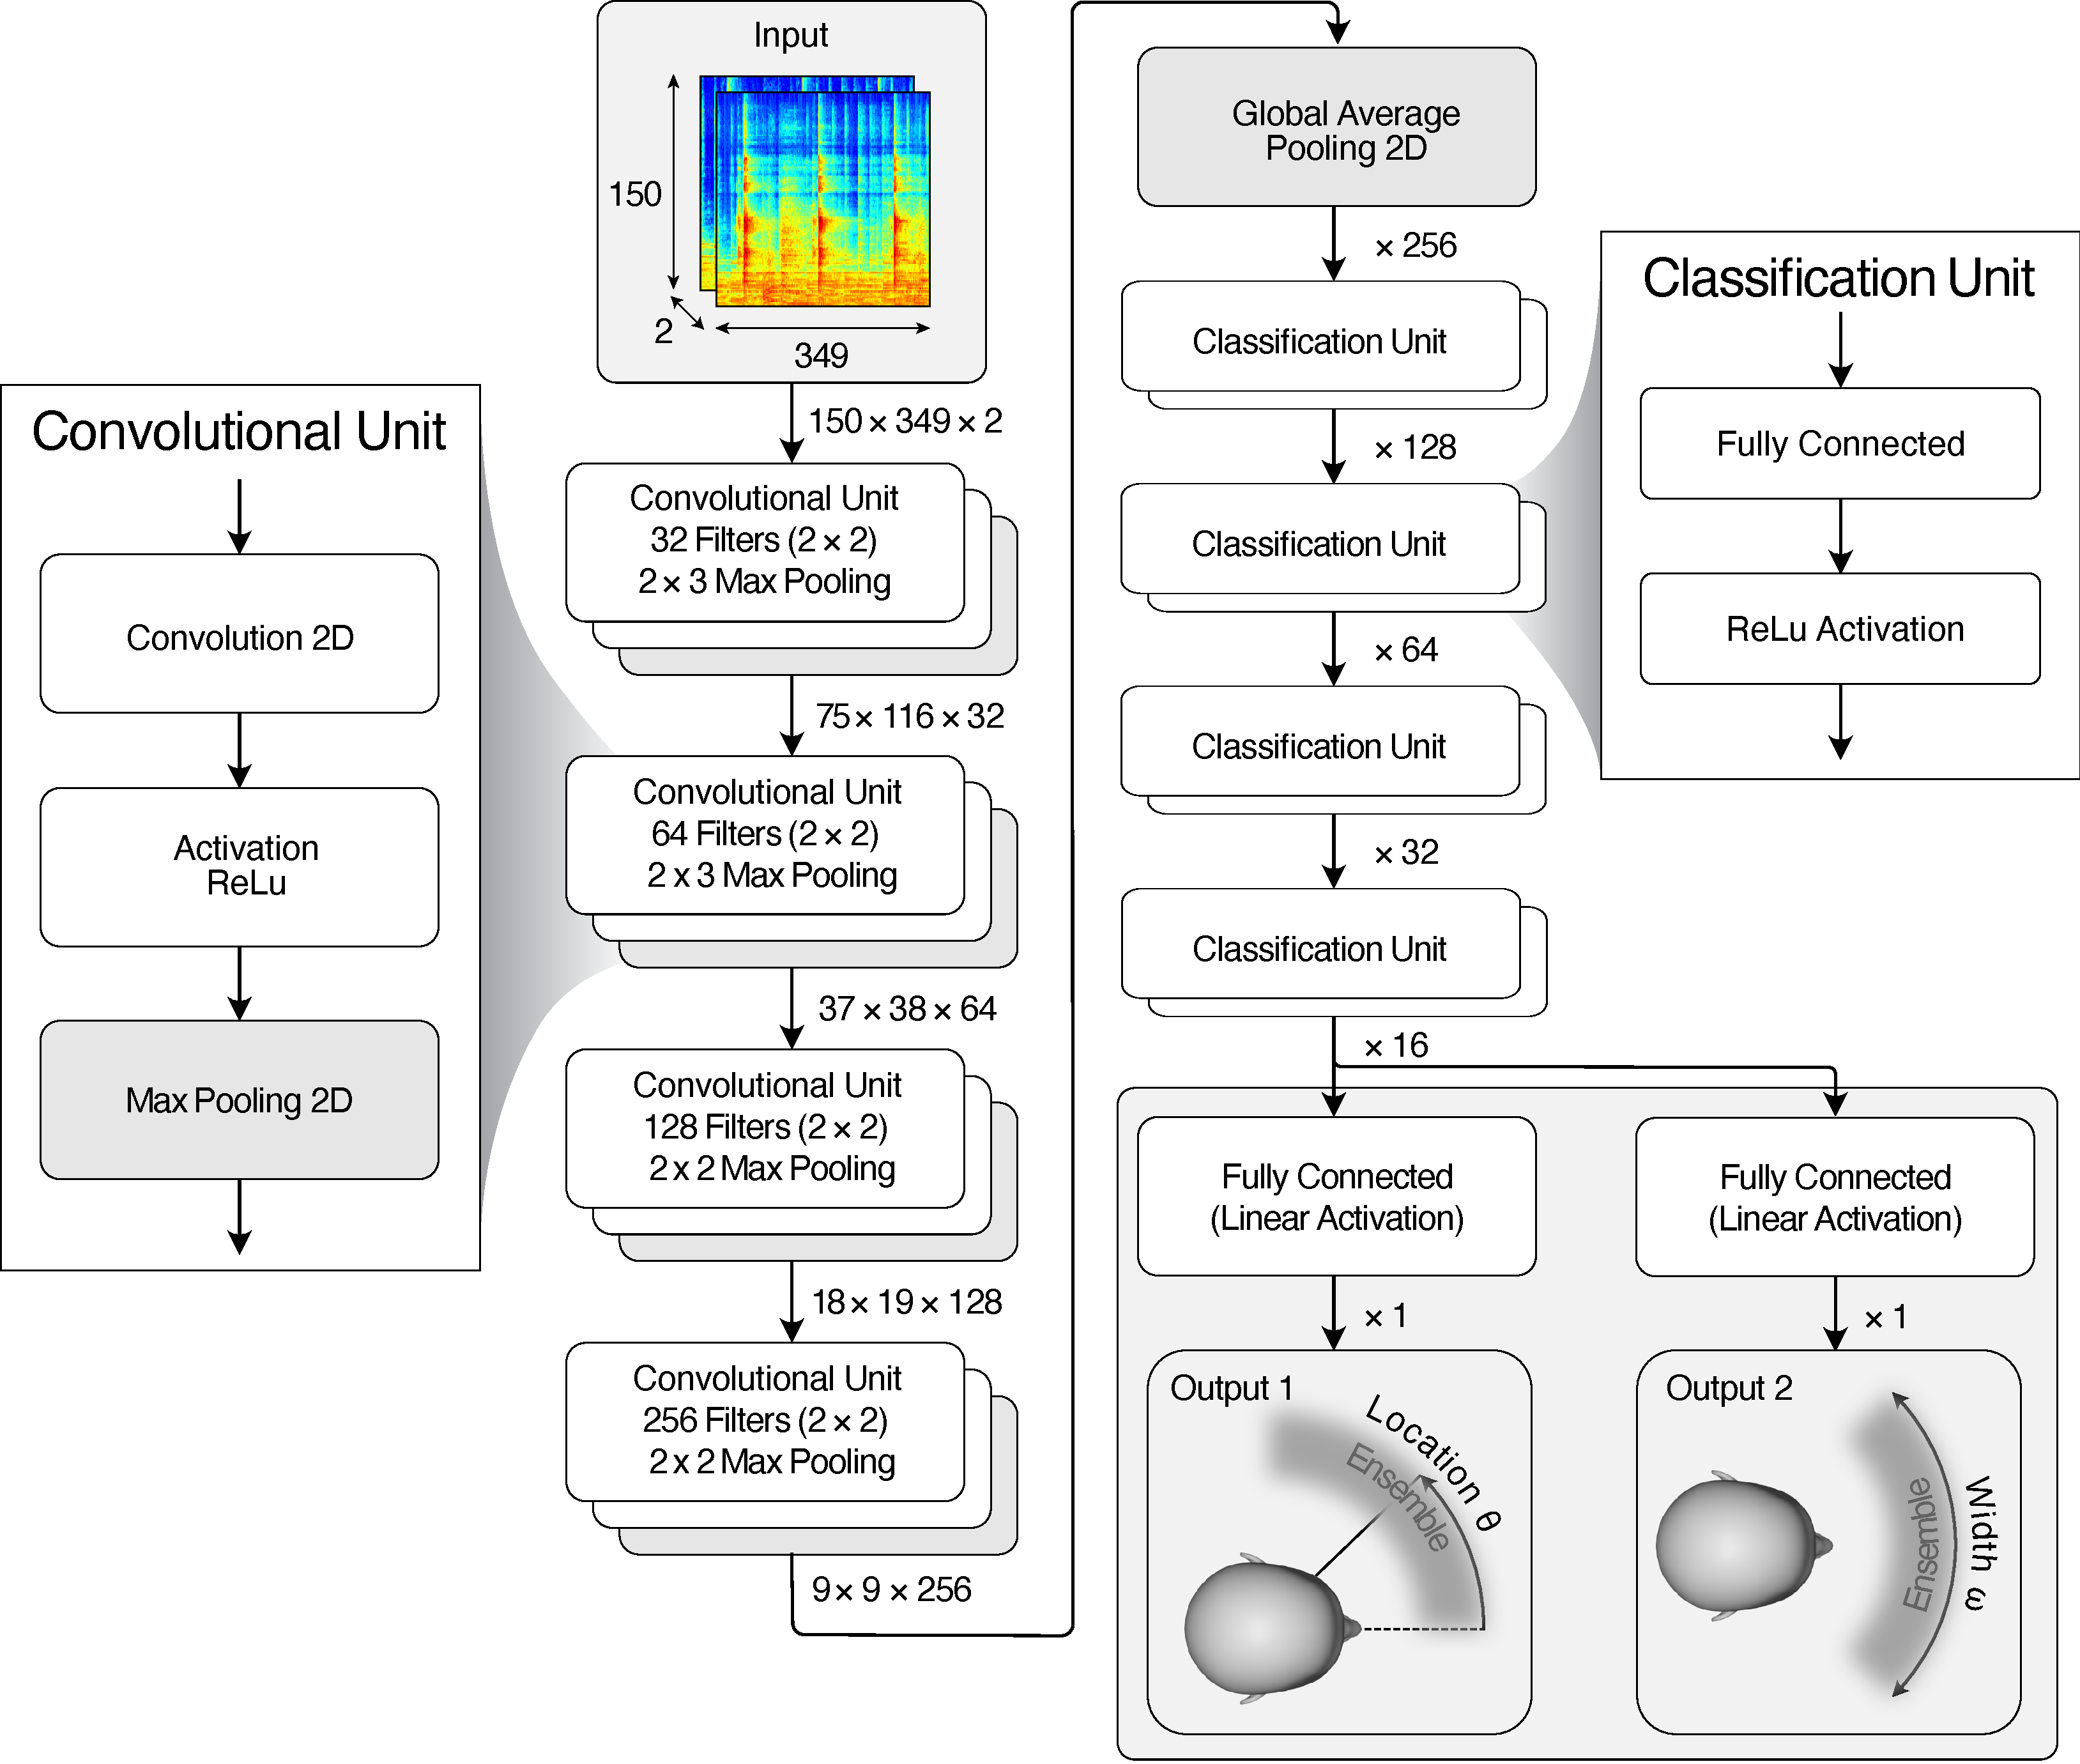
\includegraphics[width=\linewidth]{../pictures/architecture.pdf}
  \caption{\label{fig:architecture}Topology of the Convolutional Neural Network (CNN) used for identifying ensemble location and width}
\end{figure}

The network topology employed in this study was heavily influenced by the AlexNet convolutional neural network introduced by \cite{krizhevsky_imagenet_2012}. While AlexNet was originally designed for image classification, it was adapted for the audio prediction task in this study by converting binaural recordings into magnitude spectrograms, as described in Section \ref{subsec:feature_extraction}. This conversion allowed the spectrograms to be treated like images, allowing them to be used in a standard image-recognition-like task.

As illustrated in Figure \ref{fig:architecture}, the network architecture consists of an input layer accepting a pair of spectrograms, followed by a series of convolutional units and classification units, culminating in two output heads for predicting ensemble width and location. This design employs a multi-task approach, enabling a single network to predict both ensemble parameters simultaneously.

The topology finalized in this study was constructed by selecting from many alternative architectures, choosing the one with the highest prediction quality observed on the validation dataset. Despite the existence of numerous algorithms for automatic topology selection \parencite{branke_evolutionary_1995, zhang_finding_2018, miikkulainen_evolving_2017, stanley_evolving_2002, shafiee_deep_2016}, the final topology was determined manually, primarily due to the high computational demands relative to the available resources.

Various architectural configurations were assessed, with key parameters being varied such as the number of convolutional layers (from 1 to 5), the number of classification units (from 1 to 5), the inclusion or exclusion of Max Pooling Layers after each Convolution Layer, the number of filters within the Convolution Layers, the dimensions of these filters ($2 \times 2$, $2 \times 3$, or $3 \times 3$), the stride size, and the dimensions of the Max Pooling Layers ($2 \times 2$, $2 \times 3$, or $3 \times 3$). Based on this, it was concluded that the model is robust against variations in the assessed topologies. The differences in mean prediction error among the configurations were minimal, typically less than $1\degree$ for most configurations. Among the many tested topologies that yielded similar errors, the simplest one was selected to optimize both performance efficiency and model simplicity.

Despite the availability of widely used techniques for addressing overfitting, such as the Dropout Layer \parencite{srivastava_dropout_2014}, and for accelerating training, such as Batch Normalization \parencite{ioffe_batch_2015}, neither technique was employed in this study as they were observed to be ineffective for the specific prediction task being undertaken. Instead, a Global Average Pooling Layer was utilized, known for its capabilities in reducing overfitting \parencite{lin_network_2013}. This was confirmed in this particular task, as the inclusion of this layer significantly reduced overfitting, lowering the final mean absolute error score by $0.83\degree$ (average across 10 trials) compared to configurations using a Flattening Layer.

\subsection{Model training and evaluation}
\label{subsec:training_evaluation}

The topology described in the previous section resulted in a model with 216,562 learning parameters. This model training procedure was repeated 10 times, employing the Monte Carlo cross-validation method \parencite{kuhn_applied_2013}. For each repetition, the entire dataset was randomly divided into two parts: a development set containing two-thirds of the dataset (15,360 recordings) for model construction, and a test set consisting of the remaining one-third (7,680 recordings) for evaluation.

To ensure that the evaluation process was unbiased, this division was done in such a way that no original multi-track recordings used for synthesis were included in both the development and test sets simultaneously. However, this rule was not applied to HRTFs databases, allowing for the possibility of HRTF information leaking between the development and test sets. This could be seen as a significant limitation of the study. However, it is known that a human auditory system uses a single HRTF represented by ears and head, only slightly changing throughout the entire life, mainly during infancy \parencite{clifton_growth_1988, king_how_2001}, so this limitation could be considered in pair how the human auditory system behaves in the real life. Conversely, there are studies that do not implement such a limitation and test binaural localization models in an HRTF-independent manner \parencite{zielinski_spatial_2022, zielinski_automatic_2022,antoniuk_blind_2023}.

The development set was divided into training and validation subsets at a 7:1 ratio, with 13,440 recordings in the training subset and 1,920 recordings in the validation subset. The training subset was used to update the model's learning parameters, while the validation subset was solely used for early stopping \parencite{pocock_practical_1989, morgan_generalization_1989} and model checkpointing \parencite{eisenman_check-n-run_2020}, which were used for selecting the model with the best generalization capabilities and preventing overfitting. The test subset, which included data not seen during the training or validation phases, was used solely for performance assessment once per a repetition. This divide-train-and-evaluate process was repeated to collect 10 mean absolute errors, from which the final model error was determined.

For each sample, the model received two spectrograms as input: one for the left channel and one for the right channel. The rationale behind the application of Convolutional Neural Networks (CNNs) to this task was to automatically extract local features from the spectrograms and use these features to predict two contiguous ensemble parameters: ensemble location and width, both measured in degrees. The prediction errors, calculated as the difference between the actual ensemble parameters (known a priori from the binaural synthesis described in Section \ref{subsec:synthesis}) and the predicted values, were used in the Adam optimization algorithm \parencite{kingma_adam_2014}. During training, the losses for both outputs were combined by summing them, thereby treating both ensemble features with equal importance.

The computational work for this study was conducted on a workstation equipped with an RTX Nvidia GeForce 4090 GPU and a 48-core AMD Ryzen ThreadRipper processor. On the software side, MATLAB \parencite{MATLAB} with the Audio Toolbox \parencite{MATLAB_Audio_Toolbox} was used for the binaural recording synthesis, while Python \parencite{python} with the SciPy package \parencite{2020SciPy-NMeth} was used for feature extraction and Keras \parencite{chollet2015keras} for training the CNN model. The complete source code for all stages is publicly available on the GitHub repository \parencite{github_repo}. The feature extraction phase required 21 minutes, data partitioning took 34 minutes, and the total training time for all iterations was 40 minutes, making the entire training and evaluation process 95 minutes long.

\section{Results \& discussion}
\label{sec:results}

% jak uzyskane wyniki koresponduja z literatura: w jjednym przypadku ejst lepsza niz metoda oparta na spatiogramach, a w drugim przypadku nie ma 

The overall model performance measured across 10 experiment iterations, expressed as mean absolute error (MAE), was equal to $8.57\degree$ ($\pm0.19\degree$) for ensemble width and $4.76\degree$ ($\pm0.10\degree$) ensemble location. As both ensemble parameters were constrained within the same range of $90\degree$, the results demonstrate that the model exhibits a $44\%$ higher accuracy for ensemble location estimation than for ensemble width. This outcome is not unexpected, given that ensemble location is a less complex parameter. Essentially, it represents the average location of all sources. Therefore, it is more resistant to temporal fluctuations in individual audio sources than ensemble width, which is dependent on the two most extreme sound sources that vary over time. Furthermore, predicting ensemble width necessitates the identification of these two extreme sources, a process that is inherently more complex than estimating a single average location.

\begin{figure}[ht]
  \centering
  \begin{minipage}[t]{0.45\linewidth}
    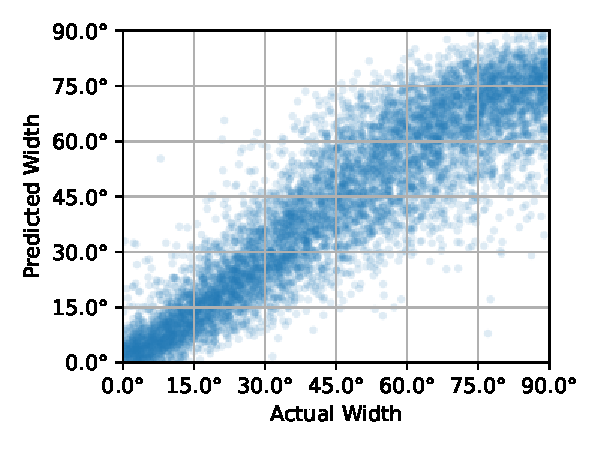
\includegraphics[width=\linewidth]{../figures/actual_vs_predicted_width.pdf}
    \caption{\label{fig:actual_vs_predicted_width}A comparison between the actual ensemble width $\omega$ and the predicted ensemble width $\omega'$ for a single iteration (of the total five) }
  \end{minipage}
  \hspace{0.5cm}
  \begin{minipage}[t]{0.45\linewidth}
    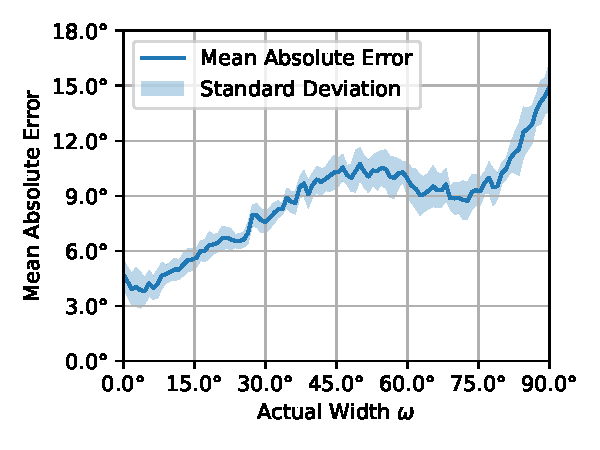
\includegraphics[width=\linewidth]{../figures/mae_width.pdf}
    \caption{\label{fig:mae_width}The impact of the actual ensemble width $\omega$ on the mean absolute prediction error, averaged across all five iterations, with indicated standard deviation.}
  \end{minipage}
\end{figure}

Figures \ref{fig:actual_vs_predicted_width} and \ref{fig:mae_width} compare the actual and predicted ensemble widths. The results indicate that the model provides more accurate predictions for narrower ensemble widths, with an average MAE of $5.65\degree$ for $\omega < 30\degree$. However, performance deteriorates as the ensemble width increases, resulting in a MAE of $12.44\degree$ for $\omega > 80\degree$. This deterioration highlights the significant impact of ensemble width on the accuracy of width estimation, particularly for wider ranges. In contrast, when comparing predicted locations to actual ones, the error remains relatively stable, as shown in Figures \ref{fig:actual_vs_predicted_location} and \ref{fig:mae_location}. The  deterioration in the width prediction can be attributed to the sparse distribution of audio sources in wider ensembles, which amplifies the influence of extreme sound sources on prediction errors, resulting in greater inaccuracies as the ensemble width increases. Moreover, Figure \ref{fig:mae_width} reveals that the relationship between the ensemble width and the error is nonlinear, displaying a notable decrease in error between $60\degree$ and $75\degree$. The reason for this nonlinearity is currently unclear and requires further investigation.

% This observed depression is in pair with other related studies, like \cite{antoniuk_blind_2023,zielinski_comparison_2020}

\begin{figure}[ht]
  \centering
  \begin{minipage}[t]{0.45\linewidth}
    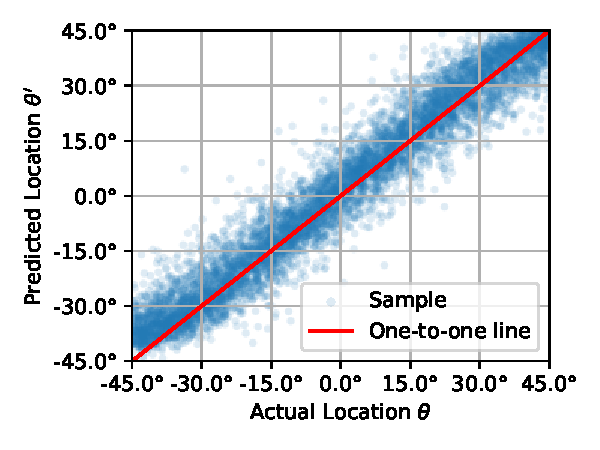
\includegraphics[width=\linewidth]{../figures/actual_vs_predicted_location.pdf}
    \caption{\label{fig:actual_vs_predicted_location}A comparison between the actual ensemble location $\theta$ and the predicted ensemble location $\theta'$ for a single iteration (of the total five) }
  \end{minipage}
  \hspace{0.5cm}
  \begin{minipage}[t]{0.45\linewidth}
    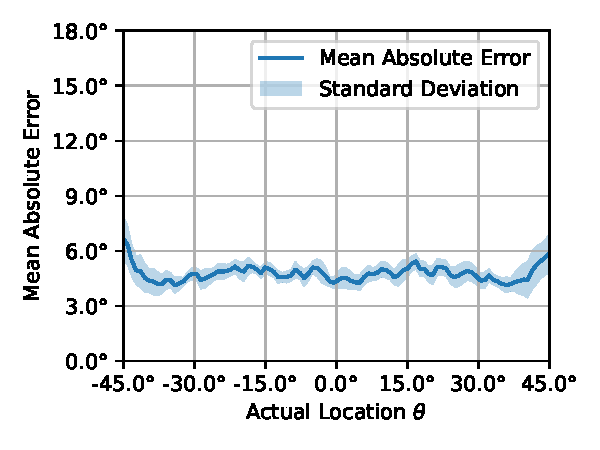
\includegraphics[width=\linewidth]{../figures/mae_location.pdf}
    \caption{\label{fig:mae_location}The impact of the actual ensemble width $\omega$ on the mean absolute prediction error, averaged across all five iterations, with indicated standard deviation.}
  \end{minipage}
\end{figure}

In contrast to the correlation between ensemble width and its prediction error, there is no significant relationship between the actual location and its prediction error, as illustrated in Figures \ref{fig:actual_vs_predicted_location} and \ref{fig:mae_location}. This finding indicates that the model's capabilities for localizing the center of the ensemble is more robust, unaffected by the actual spatial positioning of the ensemble, including lateral locations.

\begin{figure}[ht]
  \centering
  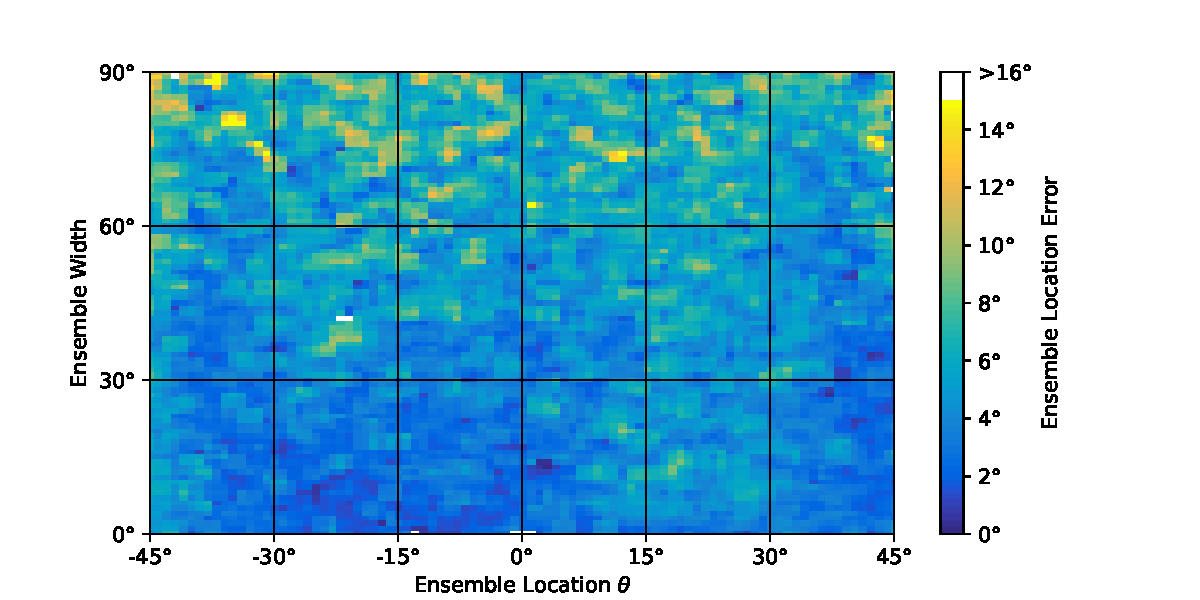
\includegraphics[width=\linewidth]{../figures/map_mae_location.pdf}
  \caption{\label{fig:map_mae_location}The heatmap that illustrates the mean absolute error (MAE) of ensemble location distribution across different ensemble locations (x-axis) and ensemble widths (y-axis). The color intensity corresponds to the MAE values, with lighter areas indicating higher errors.}
\end{figure}

\begin{figure}[ht]
  \centering
  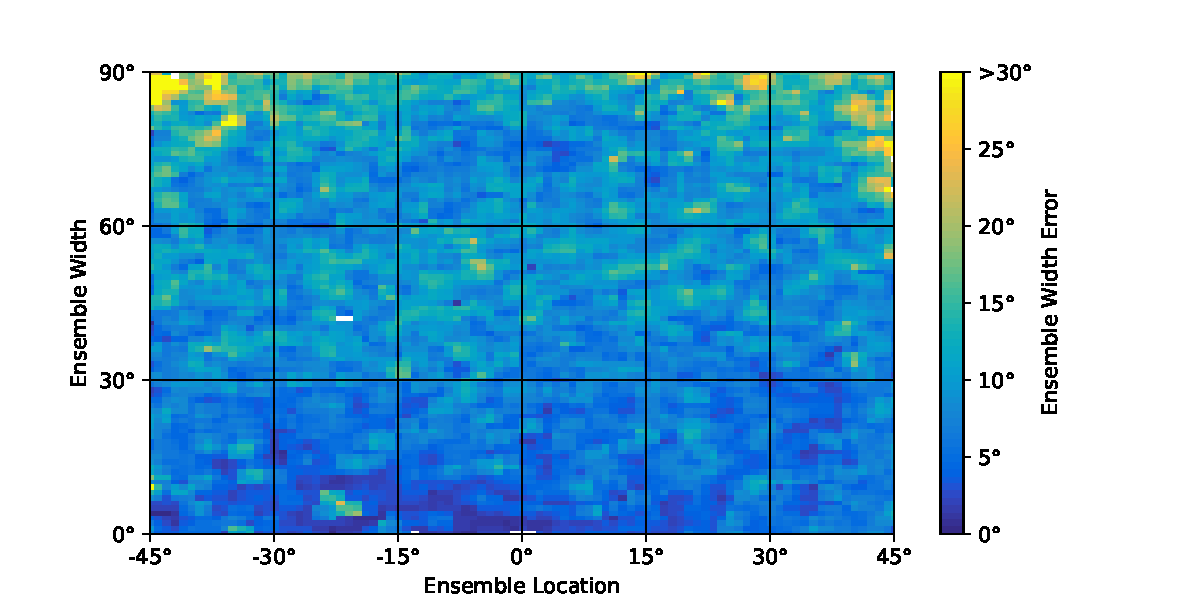
\includegraphics[width=\linewidth]{../figures/map_mae_width.pdf}
  \caption{\label{fig:map_mae_width}The heatmap that illustrates the mean absolute error (MAE) of ensemble width distribution across different ensemble locations (x-axis) and ensemble widths (y-axis). The color intensity corresponds to the MAE values, with lighter areas indicating higher errors. Notably, the values between $30\degree$ and $60\degree$ on the y-axis exhibit unexpectedly higher MAE values region --- please see Figure \ref{fig:mae_width} for comparison. }
\end{figure}

Figure \ref{fig:map_mae_location} illustrates the influence of both ensemble location and width on the mean absolute error for ensemble location, providing a detailed perspective complementing the results presented in Figure \ref{fig:mae_location}. Notably, the figure highlights some asymmetric anomalies, especially within the $\theta \in [15\degree, 30\degree]$ range compared to the $\theta \in [-30\degree, -15\degree]$ range. These anomalies can be attributed to the sparsity of sample result data across this heatmap. While the figure indicates that ensemble location does not significantly affect the model's location prediction accuracy, it clearly shows that ensemble width has a substantial impact. Similarly, Figure \ref{fig:map_mae_width} reveals a characteristic depression in $\omega \in [30\degree, 60\degree]$ previously shown from a different perspective in Figure \ref{fig:mae_width}. This heatmap highlights another interesting phenomenon in its upper corners --— the error in these areas is considerably higher. This indicates that the model's performance for estimating ensemble width is substantially worse at extreme widths and locations, i.e., when both the width and locations are at their maximum.

The achieved model's performance was better to the model based on Spatiograms \parencite{arthi_spatiogram_2021}, which performance was further investigated by \cite{antoniuk_blind_2023} within the same evaluation scenario, using the same dataset, thus making it possible to compare these two results directly. The Spatiogram-based model achieved result of $13.62\degree$, making the model presented in this study better by $5.05\degree$, suggesting a significant improvement in the prediction of this ensemble parameter. Furthermore, the model presented in the previous study did not predict the ensemble location, which further enhances the effectiveness of this method.

\section{Conclusions}
\label{sec:conclusions}

% 1. napisac wnioski, potem occulusion. we wnioskach odniesc sie do spatiogramach

\clearpage
\section*{Appendix A}
\label{appendix:a_hrtf}

\begin{longtblr}[
  caption = {List of HRTF sets used to synthesize binaural audio excerpts},
  label = {table:hrtfs}
  ]{
  colspec={c|c|>{\raggedright\arraybackslash}X|c|>{\raggedright\arraybackslash}X|c},
  hlines = {},
  vlines = {},
  cell{2}{5} = {r=2}{m},
  cell{2}{6} = {r=2}{m},
  cell{4}{5} = {r=4}{m},
  cell{4}{6} = {r=4}{m},
  cell{8}{5} = {r=3}{m},
  cell{8}{6} = {r=3}{m},
  cell{11}{6} = {r=2}{m},
  cell{13}{5} = {r=3}{m},
  cell{13}{6} = {r=3}{m},
  cell{16}{5} = {r=2}{m},
  cell{16}{6} = {r=2}{m},
  cell{18}{5} = {r=2}{m},
  cell{18}{6} = {r=2}{m},
  cell{20}{5} = {r=3}{m},
  cell{20}{6} = {r=3}{m},
  cell{23}{5} = {r=3}{m},
  cell{23}{6} = {r=3}{m},
  cell{28}{5} = {r=2}{m},
  cell{28}{6} = {r=2}{m},
  cell{30}{5} = {r=2}{m},
  cell{30}{6} = {r=2}{m},
  }
  \textbf{No.} & \textbf{Type} & \textbf{Head}                             & \textbf{Radius {[}m{]}} & \textbf{Source}                                                                                                                            & \textbf{Acronym} \\
  1.           & Human         & Human subject                             & 1.2                     & RWTH Aachen University \parencite{braren_high-resolution_2020}                                                                             & AACHEN           \\
  2.           & Artificial    & GRAS 45BB-4 KEMAR                         & 1                       &                                                                                                                                            &                  \\
  3.           & Human         & Subject 2                                 & 1.2                     & Austrian Academy of Sciences \parencite{noauthor_hrtf-database_nodate}                                                                     & ARI              \\
  4.           & Human         & Subject 4                                 & 1.2                     &                                                                                                                                            &                  \\
  5.           & Human         & Subject 10                                & 1.2                     &                                                                                                                                            &                  \\
  6.           & Artificial    & ARI Printed Head                          & 1.2                     &                                                                                                                                            &                  \\
  7.           & Human         & Subject 012                               & 1                       & CIPIC Interface Laboratory, University of California \parencite{algazi_cipic_2001}                                                         & CIPIC            \\
  8.           & Human         & Subject 015                               & 1                       &                                                                                                                                            &                  \\
  9.           & Human         & Subject 020                               & 1                       &                                                                                                                                            &                  \\
  10.          & Artificial    & Neumann KU 100                            & 0.9                     & NASA (2007) \parencite{andreopoulou_inter-laboratory_2015}                                                                                 & CLUBFRITZ        \\
  11.          & Artificial    & Neumann KU 100                            & 1.5                     & Helsinki University of Technology (2009) \parencite{andreopoulou_inter-laboratory_2015}                                                    &                  \\
  12.          & Artificial    & FABIAN                                    & 1.47                    & Technical University Berlin, Huawei Technologies, Munich Research Centre, Sennheiser Electronic \parencite{brinkmann_cross-evaluated_2019} & HUTUBS           \\
  13.          & Human         & Subject pp2                               & 1.47                    &                                                                                                                                            &                  \\
  14.          & Human         & Subject pp3                               & 1.47                    &                                                                                                                                            &                  \\
  15.          & Human         & Subject 1003                              & 1.95                    & IRCAM, AKG \parencite{noauthor_listen_2023}                                                                                                & LISTEN           \\
  16.          & Human         & Subject 1002                              & 1.95                    &                                                                                                                                            &                  \\
  17.          & Artificial    & KEMAR DB-4004 (DB-061)                    & 1.4                     & MIT \parencite{gardne_hrtf_1994}                                                                                                           & MIT              \\
  18.          & Artificial    & KEMAR DB-4004 (DB-065)                    & 1.4                     &                                                                                                                                            &                  \\
  19.          & Human         & Subject 001                               & 1.5                     & Tohoku University \parencite{watanabe_dataset_2014}                                                                                        & RIEC             \\
  20.          & Human         & Subject 002                               & 1.5                     &                                                                                                                                            &                  \\
  21.          & Artificial    & Koken SAMRAI                              & 1.5                     &                                                                                                                                            &                  \\
  22.          & Artificial    & Neumann KU 100                            & 1.2                     & University of York \parencite{armstrong_perceptual_2018}                                                                                   & SADIE II         \\
  23.          & Human         & Subject H3                                & 1.2                     &                                                                                                                                            &                  \\
  24.          & Human         & Subject H4                                & 1.2                     &                                                                                                                                            &                  \\
  25.          & Artificial    & KEMAR                                     & 1                       & South China University of Technology \parencite{yu_near-field_2018}                                                                        & SSCUT            \\
  26.          & Artificial    & Neumann KU 100                            & 1                       & TH Köln  \parencite{porschmann_spherical_2017}                                                                                             & STH Köln         \\
  27.          & Artificial    & FABIAN                                    & 1.7                     & TU Berlin \parencite{brinkmann_high_2017, wierstorf_free_2011}                                                                             & TU Berlin        \\
  28.          & Artificial    & GRAS 45BA KEMAR                           & 1                       &                                                                                                                                            &                  \\
  29.          & Artificial    & GRAS 45BB-4 KEMAR - subject A attachment  & 1                       & Aalborg University; University of Iceland \newline \parencite{spagnol_viking_2019,spagnol_viking_2020}                                     & VIKING           \\
  30.          & Artificial    & GRAS 45BB-4 KEMAR - subject B attachments & 1                       &                                                                                                                                            &                  \\
\end{longtblr}

\printbibliography

\end{document}

